\documentclass{article}


\usepackage[english]{babel}

\usepackage[letterpaper,top=2cm,bottom=2cm,left=3cm,right=3cm,marginparwidth=1.75cm]{geometry}

% Useful packages
\usepackage{amsmath}
\usepackage{graphicx}
\usepackage[colorlinks=true, allcolors=blue]{hyperref}

\title{My Paper}
\author{Tianmu Gao}

\begin{document}
\maketitle

\begin{abstract}
My abstract.
\end{abstract}

\section{Introduction}


\section{Related Work}
\subsection{Related Work}
Let $X_1, X_2, \ldots, X_n$ be a sequence of independent and identically distributed random variables with $\text{E}[X_i] = \mu$ and $\text{Var}[X_i] = \sigma^2 < \infty$\cite{1}, and let
\[S_n = \frac{X_1 + X_2 + \cdots + X_n}{n}
      = \frac{1}{n}\sum_{i}^{n} X_i\]
denote their mean. Then as $n$ approaches infinity, the random variables $\sqrt{n}(S_n - \mu)$ converge in distribution to a normal $\mathcal{N}(0, \sigma^2)$.

\section{Method}


\begin{figure}[ht]
\centering
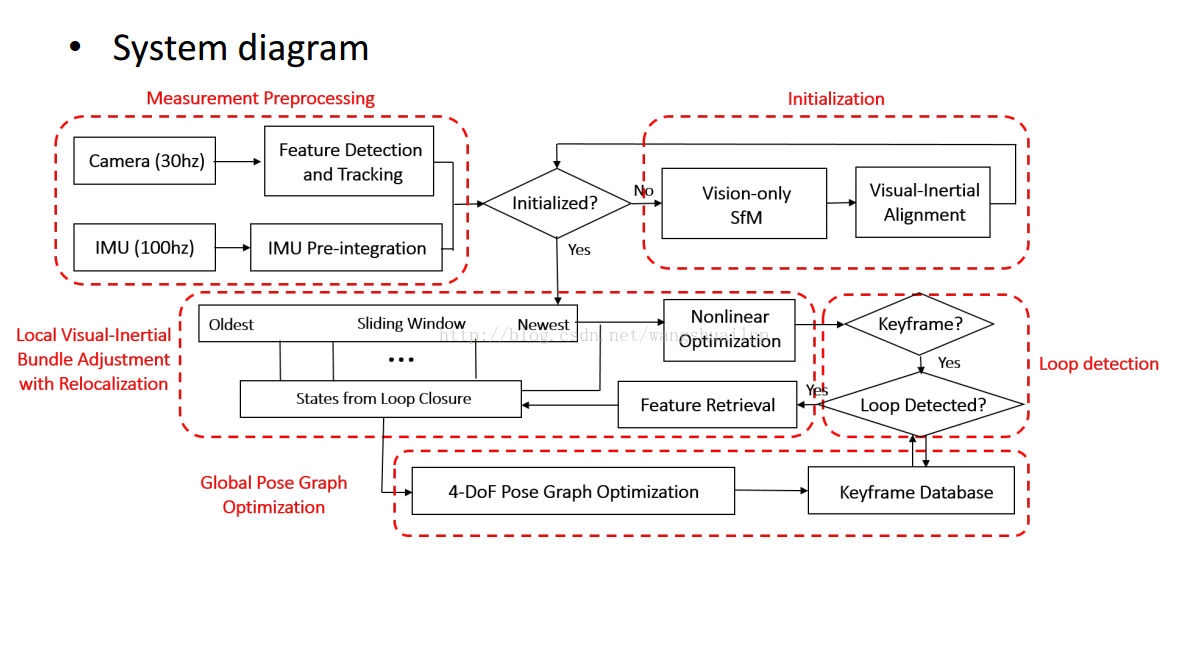
\includegraphics[width=0.8\textwidth]{vins.jpg}
\caption{\label{fig:vins}This is the structure of vins-mono.}
\end{figure}


\begin{table}[h]
\centering
\begin{tabular}{l|r}
Item & Quantity \\\hline
Widgets & 42 \\
Gadgets & 13
\end{tabular}
\caption{\label{tab:widgets}An example table.}
\end{table}

\section{Experiments}

\section{Discussion}

\begin{enumerate}
\item aaa
\item bbb
\end{enumerate}

\begin{itemize}
\item Like this,
\item and like this.
\end{itemize}

\section{Conclusion}

\bibliographystyle{IEEEtran}
\bibliography{example}

\end{document}
